\chapter{Architettura del sistema}
\label{cap:architettura}

\begin{figure}[htbp]
	\centering
	\begin{tikzpicture}[
			block/.style={rectangle, draw, rounded corners, minimum width=3.6cm,
					minimum height=1cm, align=center, fill=blue!8, font=\small},
			onetime/.style={rectangle, draw, dashed, rounded corners, minimum width=3.6cm,
					minimum height=1cm, align=center, fill=orange!10, font=\small},
			store/.style={cylinder, draw, shape border rotate=90, aspect=0.25,
					minimum height=1.6cm, minimum width=2.8cm, align=center, fill=gray!10, font=\small},
			input/.style={rectangle, draw, rounded corners, minimum width=3.2cm,
					minimum height=0.9cm, align=center, fill=green!8, font=\small},
			arrow/.style={thick, -{Latex[length=2mm]}},
		]

		% --- Input (riga y=0) ---
		\node (ropa) [input] at (0,0)   {ROPA\\(registro dei trattamenti)};
		\node (fs)   [input] at (6,0)   {File system\\/ documenti};

		% --- Blocchi una tantum (riga y=-2.4) ---
		\node (b1) [onetime] at (0,-2.4) {B1\\Normalizzazione ROPA\\(+ AI selettiva)};
		\node (b2) [onetime] at (6,-2.4) {B2\\Analisi struttura FS\\(+ AI selettiva, una tantum)};

		% --- Pipeline ricorrente (colonna destra, righe successive) ---
		\node (b3) [block] at (6,-4.8) {B3\\Estrazione \& normalizzazione\\testo};
		\node (b4) [block] at (6,-7.2) {B4\\Pipeline ibrida detection\\(regex + NER + AI selettiva)};

		% --- Persistenza / associazione (riga y=-9.6) ---
		\node (b6) [block] at (0,-9.6) {B6\\Associazione\\documento--trattamento};
		\node (b5) [store] at (6,-9.6) {B5\\Registro PII\\rilevate};

		% --- Conformità e output ---
		\node (b7) [block] at (3,-12.0)  {B7\\Verifica conformità\\(retention, categorie, PII orfane)};
		\node (b8) [block] at (3,-14.4)  {B8\\Report / dashboard DPO};

		% --- Frecce: pipeline principale ---
		\draw [arrow] (ropa) -- (b1);
		\draw [arrow] (fs)   -- (b2);
		\draw [arrow] (b2)   -- (b3);
		\draw [arrow] (b3)   -- (b4);
		\draw [arrow] (b4)   -- (b5);
		\draw [arrow] (b5)   -- (b6);
		\draw [arrow] (b6)   -- (b7);
		\draw [arrow] (b7)   -- (b8);

		% --- Freccia B1 -> B6 (verticale, colonna libera) ---
		\draw [arrow] (b1) -- (b6);

		% --- Freccia B1 -> B7: corsia dedicata a sinistra, niente clipping ---
		\draw [arrow] (b1.west) -- ++(-1.2,0) |- (b7.west);

	\end{tikzpicture}
	\caption{Architettura a macro-blocchi del sistema}
	\label{fig:architettura-macro-blocchi}
\end{figure}

\begin{figure}[htbp]
	\centering
	\begin{tikzpicture}[
			block/.style={rectangle, draw, rounded corners, minimum width=3.4cm,
					minimum height=1cm, align=center, fill=blue!8, font=\small},
			decision/.style={diamond, draw, minimum width=3cm, minimum height=1.2cm,
					align=center, fill=yellow!10, font=\small, aspect=2.2},
			ai/.style={rectangle, draw, rounded corners, minimum width=3.4cm,
					minimum height=1cm, align=center, fill=orange!10, font=\small},
			io/.style={rectangle, draw, rounded corners, minimum width=4cm,
					minimum height=0.9cm, align=center, fill=green!8, font=\small},
			arrow/.style={thick, -{Latex[length=2mm]}},
		]

		% --- Nodi ---
		\node (input)   [io]       at (0,    0)    {Testo normalizzato (da B3)};
		\node (regex)   [block]    at (-3.5, -2.5) {Regex + checksum\\(IBAN, CF, \ldots)};
		\node (ner)     [block]    at ( 3.5, -2.5) {NER\\(nomi, indirizzi, \ldots)};
		\node (merge)   [block]    at (0,    -5.2) {Merge risultati\\(overlap: sorgente doppia)};
		\node (counter) [decision] at (0,    -7.8) {documento\\campionato?};
		\node (ai)      [ai]       at (6,    -7.8) {Passata AI\\(analisi contestuale)};
		\node [font=\scriptsize\itshape, align=center, anchor=north] at (6, -9.0)
		{secondo parere\\generativo (campionato)};
		\node (output)  [io]       at (0,   -10.5) {PII unificate $\rightarrow$ B5};

		% --- Motore Presidio: fornisce i detector regex e NER (merge/AI restano proprietari) ---
		\begin{scope}[on background layer]
			\node (presidio) [draw, dashed, rounded corners, fill=purple!5,
				inner sep=5mm, fit=(regex)(ner)] {};
		\end{scope}
		\node [font=\footnotesize\itshape, anchor=north west, inner sep=3pt]
		at (presidio.north west) {Presidio};

		% --- Fork: input -> regex + ner (parallelo) ---
		\coordinate (fk) at (0, -1.2);
		\draw [thick] (input.south) -- (fk);
		\draw [arrow] (fk) -| (regex.north);
		\draw [arrow] (fk) -| (ner.north);

		% --- Join: regex + ner -> merge ---
		\coordinate (jn) at (0, -4.2);
		\draw [thick] (regex.south) |- (jn);
		\draw [thick] (ner.south)   |- (jn);
		\draw [arrow] (jn) -- (merge.north);

		% --- Merge -> counter ---
		\draw [arrow] (merge.south) -- (counter.north);

		% --- Counter: No -> output ---
		\draw [arrow] (counter.south) -- node[right, font=\footnotesize]{No} (output.north);

		% --- Counter: Sì -> AI ---
		\draw [arrow] (counter.east) -- node[above, font=\footnotesize]{Sì} (ai.west);

		% --- AI -> output ---
		\draw [arrow] (ai.south) |- (output.east);

	\end{tikzpicture}
	\caption[Dettaglio del blocco B4: pipeline ibrida di rilevamento PII]{Dettaglio del blocco B4: pipeline ibrida di rilevamento PII. I detector regex e NER sono forniti da Presidio (\texttt{AnalyzerEngine}) dietro il contratto \texttt{PIIDetector}; il merge resta proprietario. Il ramo in basso a destra --- il campionamento e la passata AI contestuale --- è \emph{realizzato}: su un campione di documenti un rilevatore generativo produce candidati che entrano nel merge come terza sorgente, confermando o scoprendo PII (§\ref{sub:b4-ai-previsto}). Lo schema è una semplificazione di flusso: i candidati generativi confluiscono nel merge accanto a quelli di regex e NER, non a valle di esso.}
	\label{fig:b4-detection-pipeline}
\end{figure}

% Le figure d'apertura del capitolo restano confinate qui, prima delle sezioni.
\FloatBarrier

La figura \ref{fig:architettura-macro-blocchi} rappresenta graficamente l'intero sistema, e costituisce la ground truth per quanto riguarda la sua implementazione. I seguenti capitoli sono suddivisi seguendo rigorosamente i blocchi dell'architettura prevista dal grafico.

\section{Input del sistema}
\label{sec:input-sistema}

Prima di discutere dei componenti attivamente presenti nel sistema, è importante inquadrare quali sono gli input usati dal sistema all'inizio della pipeline di esecuzione.

\subsection{ROPA - Registro dei Trattamenti}
\label{sub:input-ROPA}
Il primo input è il \textit{Registro dei Trattamenti (ROPA)} di un'azienda. In generale, non esiste un template riconosciuto universalmente. Questa disomogeneità porta la sua complessità, per una serie di motivi:
\begin{itemize}
	\item Tipo di file: essendo un tipo di dato libero, la sua interpretazione e decisione su come salvarlo ricade sull'azienda in questione. Esistono centinaia di modi diversi per salvare un registro, ognuno dei quali richiede particolare attenzione.
	\item Sintassi di scrittura: seppur inquadrando un certo tipo di file come più adatto, è comunque difficile predirre esattamente dove il dato a noi importante (le categorie salvate, per esempio), si trovarà all'interno del file. Questa caratteristica implica l'introduzione di un tipo di complessità basata sul contesto, ambito in cui gli algoritmi tradizionali peccano in efficienza. Una strada è sicuramente l'uso di AI generativa per la comprensione completa del documento in questione e il suo adattamento. Tuttavia, questo porta numerosi problemi, che inoltre, trascendono dallo scope di questo lavoro (AI generativa per parsing dei parametri, giusto per leggere leggermente meglio un documento)
\end{itemize}

\subsection{File system}
\label{sub:input-FS}
Il secondo input del sistema rappresenta l'insieme dei file che vanno analizzati dal sistema stesso. È possibile decidere di analizzare un singolo file, oppure un'intera cartella, o più in linea con lo scope del progetto, un'intero insieme di sottocartelle, essendo che la cartella selezionata all'interno del file system rappresenta la root da cui far partire la scansione. Per semplicità, e per bacino di utenza, è stato deciso di supportare solo un sottoinsieme di tipologie di file, includendo i più utilizzati sia in ambito consumer che enterprise. Questa scelta è stata ponderata sul fatto che, garantire il supporto ad un'infinità di tipi di file, è sicuramente un'ottima feature, ma poco interessante e poco inerente con lo scope di questo lavoro. Di conseguenza, è sembrato più consono garantire il supporto ai tipi di file "scontati" quando ci si riferisce a \textit{file non strutturati}.










\section{B1 - Normalizzazione ROPA}
\label{sec:b1-ropa}
Questo blocco è responsabile per la lettura e trasformazione del registro dei trattamenti in una forma standardizzata del sistema. Questo passaggio è obbligatorio, in quanto il termine di paragone per la verifica di conformità è tra il Registro dei Trattamenti e le PII identificate nei documenti: senza una struttura fissa e standardizzata, un confronto sarebbe estremamente dispendioso e complesso.

È stata effettauta una scelta ponderata per quanto riguarda lo schema della struttura dati che avrebbe contenuto i ROPA. Si sono presentate due possibili strade:
\begin{itemize}
	\item Struttura dati definita a monte: viene imposto uno schema noto e il database viene popolato in maniera deterministica partendo dal ROPA in input.
	\item Struttura scelta da un agente di intelligenza artificiale: il ROPA viene fornito al modello, delegando a lui la creazione della struttura del database, in base al contesto e a ciò che reputa migliore per il salvataggio in maniera efficiente dei dati.
\end{itemize}
È stata adottata la prima opzione per il seguente motivo: un Registro dei trattamento è un documento di conformità \textbf{legale}. Bisogna predilire affidabilità e riproducibilità nella sua creazione. Un modello di AI, seppur potenzialmente in grado di fornire informazioni aggiuntive, può essere soggetto ad allucinazioni o a risultati non riproducibili, casistiche non tollerabili per questi contesti.

Avere uno schema esplicito garantisce che il database sia interrogabile in maniera prevedibile dal blocco di confronto B7 (\ref{sec:b7-verifica-compliance-PII}) e mantenibile nel tempo.

L'AI non viene esclusa, ma spostata in un ambito più creativo durante la creazione del database del registro dei trattamenti (\ref{DA METTERE}).

\subsection{Template registro CNIL}
\label{sub:B1-cnil}
Per fronteggiare al problema dell'inesistenza di un template universalmente condiviso a livello mondiale o europeo per i Registri dei Trattamenti, è stato deciso di adottare come template supportato quello fornito dalla \textit{Commission Nationale de l'Informatique et des Libertés (CNIL)}, autorità di controllo francese che mette a disposizione online una versione basilare ma completa, per aiutare le azienda ad orientarsi nella creazione del proprio registro ~\cite{cnilRegistreTraitement, cnilRegistreModeleBasique}.

Questo modello è organizzato per attività di trattamento: un foglio Excel per ogni trattamento, con i seguenti campi.
\begin{itemize}
	\item identificazione del trattamento (nome, date di creazione e aggiornamento, base giuridica);
	\item attori: titolare del trattamento, eventuali co-titolari, responsabile della protezione dei dati (DPO), responsabili del trattamento esterni (\textit{processors});
	\item finalità del trattamento;
	\item categorie di persone interessate;
	\item categorie di dati personali, con evidenziazione delle categorie particolari (dati sensibili);
	\item categorie di destinatari (interni, esterni, responsabili esterni);
	\item trasferimenti verso Paesi terzi (destinazione e garanzie);
	\item durate di conservazione;
	\item misure di sicurezza tecniche e organizzative.
\end{itemize}

Per lo scopo del lavoro, \textbf{non verranno salvati tutti i dati} presenti in un trattamento. Questa scelta è stata fatta per ridurre la complessità ed evitare di salvare dati potenzialmente sensibili all'interno del database del sistema, senza un vero e proprio scopo. Di conseguenza, gli unici dati che sistematicamente vengono salvati sono quelli presenti nelle sezioni:
\begin{itemize}
	\item identità del trattamento;
	\item categorie di dati personali.
\end{itemize}

% qui da valutare se mettere la discussione con relatore
La struttura scelta per rappresentare il registro segue la sua gerarchia naturale su \textbf{tre livelli}. Al primo, l'\textbf{attività di trattamento}, con la sua identità (un nome e una finalità). Al secondo, i \textbf{blocchi di categorie} che vi appartengono, ciascuno con la propria \textbf{durata di conservazione}, che le categorie raccolte nel blocco ereditano. Al terzo, le \textbf{singole categorie dichiarate}, ognuna ricondotta al vocabolario condiviso delle categorie di PII --- lo stesso usato dal rilevamento (B4). È quest'ultimo aggancio a rendere il confronto fra ciò che il registro \emph{dichiara} e ciò che il motore \emph{rileva} (B7) una semplice operazione insiemistica: e una categoria che non si risolve in alcun tipo rilevabile resta \textbf{esplicita} nel modello --- dichiarata ma non verificabile dal motore --- e come tale va segnalata al DPO, non scambiata per conforme. La durata di conservazione, infine, è tenuta accanto al testo originale in forma \emph{confrontabile dalla macchina}, così che il superamento del termine (B7) sia \emph{calcolato} al momento del controllo e non registrato come stato. La resa concreta di questo modello --- tabelle, campi e tipi --- è nella sezione di implementazione (§\ref{sec:dati-persistiti}).


\subsection{Ruolo AI in ROPA}
\label{sub:B1-AI}

Il popolamento dei primi due livelli del modello --- l'attività di trattamento e i blocchi di categorie --- è deterministico: la struttura CNIL è nota e i campi si trasferiscono direttamente. Il terzo livello, la singola categoria dichiarata, è invece spesso testo libero e sbrigativo («dati anagrafici, coordinate bancarie, contatti»): ricondurlo al \textbf{vocabolario condiviso delle categorie di PII} --- lo stesso che il rilevamento (B4) usa --- richiede un'interpretazione contestuale, per la quale un algoritmo puramente sintattico è inadeguato. È l'unico punto dell'ingestione in cui interviene un modello generativo, ed entro due vincoli architetturali stretti. Primo, è un intervento \textbf{circoscritto}: una volta, a livello di singolo campo, per scindere ed espandere un testo libero in categorie normalizzate --- non una delega della struttura del documento, coerente con la scelta \emph{non agentica} del blocco. Secondo, opera dentro un \textbf{vocabolario chiuso}: ogni categoria proposta è validata contro quel catalogo condiviso, e una proposta che non vi rientra è scartata, sicché il modello non può introdurre categorie che il sistema non sa rilevare.

Soprattutto, l'esito del modello è una \emph{proposta}, non una decisione: la mappatura resta tale finché il DPO non la conferma. È l'istanza, in questo blocco, di un principio che attraversa l'intero sistema: qualunque sia l'origine di un'inferenza --- un dizionario deterministico, un modello generativo, una regola che associa una cartella a un trattamento, la segnalazione di una PII orfana --- l'atto che la rende parte della \emph{verità dichiarativa} è sempre umano. Il sistema propone, il DPO dispone. È il gemello, sul versante della decisione, dei principi di \emph{recall-first} e di \emph{minimizzazione}: come quelli evitano rispettivamente di scartare e di trattenere, questo evita di \textbf{decidere al posto dell'umano}. La realizzazione --- i due mapper intercambiabili, il prompt, la validazione, la conferma --- è descritta in §\ref{sub:impl-b1-mappatura}.
















% ============================================================================
% SCAFFOLDING (temporaneo) — mappa parallela §6 (idea) <-> §7 (realizzazione).
% Struttura dati DENTRO i blocchi. In §6 il lavoro e' quasi tutto RECUPERO dalle
% vecchie sezioni tematiche piu' in basso (237+): svuotarle in questi stub e poi
% cancellarle. Eliminare questo scaffold a lavoro finito.
% ----------------------------------------------------------------------------
% B2 - Analisi struttura FS (NON realizzato)
%   §6: perche' previsto e non fatto (l'utile e' gia' dato dalle regole
%       cartella->trattamento, B6). Recuperare da: §"Un blocco previsto e non
%       realizzato" (piu' in basso).  |  §7: nulla (non implementato).
% ----------------------------------------------------------------------------
% B3 - Estrazione e normalizzazione del testo
%   §6 (idea): estrazione born-digital -> testo normalizzato; la DATA DI
%       RIFERIMENTO con provenienza (metadati->mtime) come dato del blocco;
%       niente OCR/layout. Recuperare da: §"Livello di estrazione del testo".
%   §7 (come): lettori PDF/DOCX/txt + fogli + .doc legacy; extraction/dates.py
%       (catena metadati->mtime, guardia <1990/futuro, degrado grazioso).
%   struttura inline (§6): il documento normalizzato + reference_date con la fonte.
% ----------------------------------------------------------------------------
% B4 - Pipeline ibrida di detection
%   §6 (idea): due sorgenti dietro PIIDetector + il merge (4 casi) + il ramo
%       generativo. GIA' SCRITTO piu' in basso (§"Livello di rilevamento ibrido":
%       sorgenti / merge / ramo AI) -> SPOSTARE qui.
%   §7 (come): Presidio pattern+NER, GLiNER, RegexDetector config-driven (gia' in
%       §7), LLMDetector (prompt, valore->span, chunking, never-raise), MergeEngine,
%       slot opzionale ai + AITriggerPolicy.
%   struttura inline: PIICandidate -> PIIMatch (span, tipo, confidence, livello, sorgenti).
% ----------------------------------------------------------------------------
% B5 - Registro PII rilevate
%   §6 (idea): changelog delta-based (stato + storia); i DUE OROLOGI (data
%       semantica vs impronta tecnica); minimizzazione (mai il valore).
%       Recuperare da: §"Persistenza del registro delle PII".
%   §7 (come): 4 tabelle (document/scan/instance/change); freshness (incrementale);
%       refresh CONFIRMED. GIA' in §7 (§"Dati persistiti" -> registro PII).
%   struttura inline (§6): documento -> scansione -> istanza (stato) + variazione (log); ER concettuale.
% ----------------------------------------------------------------------------
% B6 - Associazione documento-trattamento
%   §6 (idea): associazione esplicita + regole cartella (prefisso->attivita'),
%       provenienza MANUAL/RULE; + IL PONTE CROSS-DB: due database separati, join
%       LOGICO sull'id-stringa (QUI il posto giusto per il pezzo trasversale).
%       Recuperare da: §"Associazione e verifica" -> sottosez. B6.
%   §7 (come): FolderRule, riconciliazione (azzera RULE stale), auto-apply a fine scan.
%   struttura inline: Document.activity_ids (N:N) + FolderRule(prefix->activity_ids).
% ----------------------------------------------------------------------------
% B7 - Verifica conformita' + conservazione
%   §6 (idea): confronto should/is -> orfane/coperte/mancanti; retention (eta' vs
%       termine + "non verificabile"); + DALLA PII ORFANA ALLA PROPOSTA (il
%       feedback: orphan -> categoria PROPOSED, il DPO conferma). Recuperare da:
%       §"Associazione e verifica" -> sottosez. B7 + "Verifica della conservazione".
%   §7 (come): checker.build_report; vista di corpus /retention; propose_category.
%   struttura inline (§6): il verdetto (ComplianceReport) come valore di sola lettura.
% ----------------------------------------------------------------------------
% B8 - Dashboard DPO
%   §6 (idea): restituzione al DPO; human-in-the-loop (gia' enunciato in B1);
%       Post/Redirect/Get come principio. Recuperare da: §"Interfaccia e
%       restituzione al DPO".
%   §7 (come): app FastAPI unica (una porta); pagine (dashboard / documento /
%       /retention / /scan / /rules; review ROPA montata sotto /ropa); trigger AI
%       (menu campionamento, per-documento ASINCRONO via ScanJob); due fasi;
%       indicatore di scansione attiva.
% ----------------------------------------------------------------------------
% TRASVERSALE
%   §6: nuova sezione "Pattern architetturali e di progettazione" (Strategy / DI /
%       Factory / Adapter / Composite / Policy / Active Record; l'argomento
%       Open-Closed che giustifica lo slot opzionale invece di un Registry = YAGNI).
%   §7: "Deployment containerizzato" (GIA' SCRITTO).
%   Principi trasversali, enunciati UNA volta: recall-first, minimizzazione, DPO
%   sovrano (gia' in B1).
% ============================================================================

\section{B2 - Analisi struttura File System}
\label{sec:b2-analisi-struttura}
Feature presente nell'architettura originale, ma non implementata per vincoli tempistici e di scarsa sicurezza e utilità del possibile risultato. Presente in maniera più approfondita nella sezione degli Sviluppi Futuri \ref{SEZIONE}

\section{B3 - Estrazione e normalizzazione del testo}
\label{sec:b3-estrazione-testo}

Il blocco B3 sta a monte del rilevamento: trasforma un file, in uno dei formati supportati (§\ref{sub:input-FS}), nel \textbf{testo normalizzato} su cui opererà il motore di detection. Il suo prodotto è deliberatamente semplice --- un flusso di testo lineare, spogliato della formattazione --- ed è \emph{questo}, non il documento originale, ciò che entra nel blocco B4: la medesima forma di testo è consumata allo stesso modo dai rilevatori a regole e dal modello generativo, sicché a valle nessuno deve più sapere da quale formato il documento provenisse. La normalizzazione è leggera (spazi e a-capo) e non tenta di ricostruire il \emph{layout}: il sistema tratta documenti \emph{born-digital}, non scansioni, e l'OCR resta fuori ambito (cfr.~§\ref{cap:sviluppi-futuri}).

Una scelta di progetto merita di essere resa esplicita, perché ribalta un'assunzione iniziale. L'estrazione era stata concepita attorno a uno strumento dedicato --- Docling~\cite{livathinosDoclingEfficientOpenSource2025} --- pensato per convertire formati complessi in testo pulito, fruibile tanto da un modello generativo quanto dai rilevatori a regole. All'atto dell'implementazione, però, i formati che selezionati per essere supportati si sono rivelati sufficentemente semplici da non richiedere quell'apparato: bastano conversioni leggere che riducono ogni file a un flusso di testo direttamente analizzabile. Docling resta possibile risorsa qualora l'insieme dei formati si allargasse a documenti realmente complessi (§\ref{cap:sviluppi-futuri}); allo stato attuale sarebbe complessità non ripagata. Coerentemente con la separazione fra architettura e realizzazione, le scelte implementative appartengono al capitolo di implementazione (§\ref{sec:impl-b3-estrazione}).

% ---------------------------------------------------------------------------
% Bozza mista originale (NON cancellare --- traccia da cui e' derivato il testo sopra
% e le indicazioni §6/§7; da rimuovere a lavoro finito):
% Questa registrazione serve come in base per poi scrivere il la sezione B3 per quanto riguarda l'estrazione, la normalizzazione del testo dei documenti del sistema. Questa sezione in particolare inizialmente era stata pensata per essere. Soltanto basata su dockling Una applicazione. esterna che Il suo compito è quello di convertire formati particolarmente. Complessi in testo facilmente leggibile sia da AI, ma anche da rilevatori Basati su regole come presidio, quello che viene usato nel progetto, d'altronde. Dopo però L'inizio dell'implementazione La cosa è stata più semplice del previsto in quanto i tipi di file. Che ho deciso di trattare Erano molto più primitivi di quello che mi aspettassi. Infatti. È bastato utilizzare delle librerie in Python molto più leggere e che permettevano. Di trasformare al volo il file in questione direttamente diciamo. In una streaming di testo che poteva essere molto più facilmente. Parsata dal Dal motore di rilevamento. I tipi di file supportati. Sono quelli più utilizzati a livello enterprise, a livello customer. Ma questa sezione c'è già precedentemente. sui tipi di file appunto supportati nella sezione del file system. Nella in questa sezione di architettura. Non vanno messi i nomi delle librerie in sé andranno messi poi nella sicuramente nella sezione di implementazione con anche tipo di tipo di estensione del file con. Il nome della libreria e il suo eventuale utilizzo, ovviamente senza entrare eccessivamente nel dettaglio, ma comunque è giusto. Dirlo. Quindi questo è per quanto riguarda il blocco B3. Cosa da mettere secondo me che ha senso in questa sezione qual è l'effettivo. Output di questo blocco o meglio che cosa entra direttamente nel blocco B4 della detection. Secondo me, appunto centrale. Però iniziamo a scrivere questo
% ---------------------------------------------------------------------------

\section{B4 - Pipeline ibrida di detection di PII}
\label{sec:b4-pipeline-detection}
\label{sec:rilevamento-b4}

Il blocco B4 della Figura~\ref{fig:architettura-macro-blocchi} è il motore di rilevamento vero e proprio: dato il testo già estratto e normalizzato dal blocco a monte, individua le PII presenti nel documento e le consegna, unificate, al registro (B5). È un livello \emph{ibrido}, che combina due tecniche indipendenti e complementari --- un'impostazione che la letteratura recente sul rilevamento di PII indica come la più robusta rispetto alle singole tecniche prese isolatamente~\cite{mishraHybridRulebasedNLP2025, rajgarhiaEvaluationStudyHybrid2025}; la sua architettura interna è dettagliata nella Figura~\ref{fig:b4-detection-pipeline}.

\subsection{Due sorgenti complementari dietro un contratto unico}
\label{sub:b4-sorgenti}

Le due tecniche coprono classi di PII diverse. Le \textbf{espressioni regolari}, affiancate dalla verifica di \emph{checksum} dove il formato la prevede, riconoscono gli \emph{identificatori strutturati} --- IBAN, codice fiscale, numero di carta, indirizzo IP --- dove la forma è rigida e la precisione può essere massima. Il \textbf{riconoscimento di entità nominate} (NER) copre invece i dati meno strutturati e dipendenti dal contesto --- nomi di persona, indirizzi --- dove nessuna regola fissa è sufficiente. La validazione a \emph{checksum} non è un affinamento previsto ma una proprietà già operante: un IBAN o un codice fiscale formalmente ben scritto ma incoerente nella cifra di controllo viene scartato, ed è la ragione per cui il corpus di valutazione (Cap.~\ref{cap:test}) deve generare valori \emph{aritmeticamente validi} --- altrimenti sarebbe il \emph{gold} stesso a essere respinto, gonfiando artificiosamente i falsi negativi.

Entrambe le tecniche sono esposte al resto del sistema attraverso un unico contratto, \texttt{PIIDetector} (nella forma \texttt{detect(testo)} $\rightarrow$ lista di candidati): l'orchestrazione dipende solo da questa forma, non dalla tecnologia sottostante, così una sorgente può essere sostituita senza toccare il resto del livello. Nella realizzazione le due sorgenti poggiano sul motore \textit{open source} Microsoft Presidio~\cite{HomeMicrosoftPresidio}, adottato come base per regex e NER a valle di una valutazione sperimentale (§\ref{sec:valutazione-presidio}).

\paragraph{Estendere il rilevamento senza scrivere codice.} Lo stesso contratto rende possibile \emph{comporre} più rilevatori in un unico posto della pipeline. Su questa possibilità poggia il punto di estensione richiesto dai requisiti (cfr.~§\ref{sub:estensibilita}): accanto ai riconoscitori predefiniti opera un rilevatore \textbf{guidato da configurazione}, che esegue le regole dichiarate in un file esterno. Aggiungere un identificatore proprio di un settore o di un ordinamento --- e la categoria corrispondente nel catalogo --- è quindi una modifica \emph{dichiarativa}, non un intervento sul codice sorgente. La coerenza di questa scelta è stata verificata applicandola a sé stessa: l'unico identificatore che era stato cablato nel motore come caso speciale (il numero AVS svizzero) è stato ricondotto al medesimo meccanismo, così che esista una sola strada per tutti i pattern anziché due.

\subsection{Il merge: unificazione e grado di certezza}
\label{sub:b4-merge}

Le due sorgenti producono candidati in modo autonomo; il \emph{merge} li unifica in un unico insieme di PII, decidendone il grado di certezza in base a \emph{quante} e \emph{quali} sorgenti concordano su una stessa porzione di testo. Confrontando gli span per sovrapposizione, ogni PII risultante ricade in uno di quattro casi --- un vocabolario chiuso:

\begin{itemize}
	\item \textbf{Fonte singola} --- rilevata da una sola tecnica, senza sovrapposizioni. Non viene mai scartata (cfr.\ il principio \emph{recall-first} più sotto), ma etichettata come meno certa.
	\item \textbf{Doppia conferma} --- due o più sorgenti concordano sullo stesso tipo di PII su span sovrapposti: pattern e NER, oppure l'una o l'altra insieme alla passata generativa. È il caso più solido: la confidenza viene rinforzata.
	\item \textbf{Conflitto} --- gli span si sovrappongono ma le sorgenti assegnano tipi diversi. Il merge \textbf{non arbitra}: conserva entrambe le ipotesi e demanda la risoluzione al blocco a valle, che dispone di più contesto.
	\item \textbf{Scoperta dall'AI} --- individuata dalla passata generativa selettiva (campionata), assente dalle altre sorgenti. È il caso in cui il modello generativo aggiunge qualcosa che gli algoritmi tradizionali non hanno visto (§\ref{sub:b4-ai-previsto}).
\end{itemize}

\paragraph{Principio recall-first.} Nessuna sorgente scarta di propria iniziativa un candidato debole: al più lo segnala con confidenza bassa. La ragione è la finalità di conformità del sistema: un falso positivo costa al DPO una verifica in più, mentre una PII \emph{mancata} è un rischio che resta invisibile. Il merge eredita questo principio --- non elimina, ma unifica e classifica --- lasciando ogni eventuale scarto a una decisione umana o a un blocco a valle.

\paragraph{Il ruolo della passata generativa.} La terza sorgente, quando presente, entra nel merge per ultima e vi gioca due ruoli. Se ricade su una PII già trovata e ne concorda il tipo è \emph{confermatrice}: la sua provenienza si aggiunge alle altre e la certezza sale (una fonte singola diventa a doppia conferma, una già doppia acquista una terza voce). Se cade dove nessun'altra sorgente ha visto nulla è \emph{scopritrice}, e produce il quarto caso. Il disaccordo segue lo stesso principio recall-first, ma pesato: un parere generativo singolo che contraddice un'altra fonte mette le due sullo stesso piano (entrambe in conflitto, arbitraggio a valle), ma \textbf{non basta a incrinare} un accordo già raggiunto fra pattern e NER, che resta tale. La certezza, in altre parole, non si perde per una contestazione più debole di ciò che contesta.

\paragraph{Un solo modello dato.} La PII unificata prodotta dal merge non richiede un modello dati intermedio: la sua \emph{certezza} è già descritta da tre attributi che essa porta con sé --- la confidenza (quanto è forte il rilevamento), il livello di conferma appena descritto, e l'elenco delle \emph{provenienze} (quali e quanti detector concordano, ciascuno con la propria confidenza). Mantenere questi campi sul singolo oggetto, invece di duplicarli in strutture parallele, conserva un'unica fonte di verità per la PII rilevata e ne preserva la tracciabilità verso il DPO.

\subsection{Il ramo generativo come secondo parere}
\label{sub:b4-ai-previsto}

Le due sorgenti descritte finora appartengono al paradigma degli algoritmi \emph{tradizionali}: veloci, deterministici, economici, ma ciechi a tutto ciò che non è previsto in una regola o in un'etichetta. Il ramo generativo affianca loro un modello linguistico come \emph{secondo parere}, per rispondere a una domanda che è di merito e non di ingegneria --- se e quando un modello che legge il documento come farebbe un lettore umano~\cite{brownLanguageModelsAre2020} trovi dato personale che quegli algoritmi non trovano, e se il guadagno giustifichi il suo costo, superiore di ordini di grandezza in tempo ed energia. La scelta del modello e la sua valutazione sono l'oggetto degli studi che precedono la progettazione (§\ref{sec:scelta-modello-llm}, distinzione Task 1 / Task 2 in §\ref{sub:slm-task}); l'esito comparativo è nel Capitolo~\ref{cap:risultati}.

Ciò che qui rileva è la forma architetturale, ed è dettata proprio da quella domanda: perché l'AI sia \emph{confrontabile} con le sorgenti tradizionali, va costruita come una sorgente fra le altre, non come un meccanismo a parte. Il rilevatore generativo è perciò incapsulato dietro lo stesso contratto \texttt{PIIDetector} di regex e NER, così che il merge lo accolga come terza voce (§\ref{sub:b4-merge}) e lo stesso apparato di misura che assegna precisione e richiamo a un rilevatore possa assegnarli al modello generativo senza codice speciale.

\paragraph{Quando accendere l'AI: una politica del chiamante.} Una passata generativa costa da secondi a minuti per documento, quindi non la si esegue su ogni file a ogni scansione (cfr.\ l'impiego \emph{selettivo} previsto dai requisiti, §\ref{sub:ai-selettiva}, e il costo in §\ref{sec:impatto-ambientale}). La decisione su \emph{quali} documenti sottoporre all'AI è però tenuta \textbf{fuori} dal rilevatore --- che si limita ad analizzare il testo che riceve --- e affidata a una \emph{politica} del chiamante: nessuna analisi, tutti i documenti, oppure un campione. Separare la politica dal rilevatore è ciò che consente di innescare l'AI in modi diversi (a campione durante una scansione, o su richiesta su un singolo documento) senza duplicare la logica di rilevamento. La realizzazione del rilevatore e della politica --- prompt a catalogo chiuso, difese anti-allucinazione, campionamento --- è descritta in §\ref{sec:impl-detection}.

\section{B5 - Registro PII rilevate}
\label{sec:b5-DB-PII}

\section{B6 - Associazione documento-trattamento}
\label{sec:b6-documento-trattamento}

\section{B7 - Verifica conformità PII presenti}
\label{sec:b7-verifica-compliance-PII}

\section{B8 - Dashboard per DPO}
\label{sec:b8-dashboard}

\section{Ingestione e modello dati del ROPA}
\label{sec:modello-ropa}

Il blocco B1 della Figura~\ref{fig:architettura-macro-blocchi} acquisisce il ROPA (\textit{Record of Processing Activities}, il registro delle attività di trattamento) e lo trasforma in una rappresentazione interna. Non è una fase accessoria: il ROPA è il termine di paragone \textit{atteso} rispetto al quale la verifica di conformità (B7) confronta le PII effettivamente rilevate nei documenti. La sua struttura dati condiziona quindi ciò che il sistema è in grado di verificare. Questa sezione motiva l'approccio scelto per modellarlo.

\subsection{Strutturazione a monte o delega all'AI}
\label{sub:ropa-approccio}

L'ingestione del ROPA ammette due strategie agli estremi opposti. Nella prima la \textbf{struttura dati è definita a monte}: il sistema impone uno schema noto e l'ingestione lo popola in modo deterministico a partire da un ROPA già compilato. Nella seconda, \textbf{totalmente agentica}, i documenti del ROPA vengono forniti così come sono a un modello generativo, delegando a esso l'individuazione della struttura --- l'approccio «si immettono i documenti e si osserva cosa emerge».

Si adotta la prima. Un registro dei trattamenti è un \textit{artefatto di conformità}: la sua affidabilità e la sua auditabilità non possono dipendere da una strutturazione inferita, potenzialmente allucinata e non riproducibile. Uno schema esplicito garantisce inoltre che il modello sia interrogabile in modo prevedibile dal blocco di confronto (B7) e mantenibile nel tempo. L'AI non viene esclusa, ma \textbf{circoscritta} a un ruolo di arricchimento su un singolo campo (§\ref{sub:ropa-ai}); ciò è coerente con l'uso selettivo dell'AI già previsto per il blocco B1 nella Figura~\ref{fig:architettura-macro-blocchi}.

\subsection{Il registro-tipo CNIL come schema di riferimento}
\label{sub:ropa-cnil}

Il contenuto obbligatorio del registro è fissato dall'art.~30 del Regolamento (UE) 2016/679~\cite{gdprArt30} e, per il contesto svizzero, dall'art.~12 della LPD~\cite{nlpdArt12}; i due elenchi sono ampiamente sovrapponibili. In assenza di una pluralità di modelli operativi consolidati, il riferimento pratico più diffuso è il registro-tipo pubblicato dalla \textit{Commission Nationale de l'Informatique et des Libertés} (CNIL), l'autorità di controllo francese, derivato direttamente dall'art.~30~\cite{cnilRegistreTraitement, cnilRegistreModeleBasique}. Adottarlo come base evita di progettare uno schema dal principio e lega il modello ad una fonte ampiamente autorevole e condivisa.

Il modello CNIL è organizzato per \textit{attività di trattamento}: una scheda per ciascun trattamento, con i campi seguenti.
\begin{itemize}
	\item identificazione del trattamento (nome, date di creazione e aggiornamento, base giuridica);
	\item attori: titolare del trattamento, eventuali co-titolari, responsabile della protezione dei dati (DPO), responsabili del trattamento esterni (\textit{processors});
	\item finalità del trattamento;
	\item categorie di persone interessate;
	\item categorie di dati personali, con evidenziazione delle categorie particolari (dati sensibili);
	\item categorie di destinatari (interni, esterni, responsabili esterni);
	\item trasferimenti verso Paesi terzi (destinazione e garanzie);
	\item durate di conservazione;
	\item misure di sicurezza tecniche e organizzative.
\end{itemize}

\subsection{Normalizzazione in un modello relazionale}
\label{sub:ropa-modello}

La scheda CNIL è \textit{denormalizzata} --- un foglio piatto per trattamento --- e ricca di campi che il sistema non ha motivo di modellare. Poiché la verifica di conformità (B7) confronta le categorie di dati \textit{dichiarate} con quelle \textit{rilevate}, il modello interno conserva soltanto ciò che alimenta quel confronto --- l'identità del trattamento e le sue categorie di dati personali --- e scarta deliberatamente gli altri campi della scheda (attori, categorie di interessati, destinatari, trasferimenti verso Paesi terzi, misure di sicurezza). È una scelta \textbf{sottrattiva}: riduce la superficie da mantenere e da tenere allineata alla fonte, senza togliere nulla a ciò che il sistema deve poter verificare.

Ciò che resta viene normalizzato in una gerarchia a \textbf{tre livelli}, che ricalca l'organizzazione del registro CNIL:
\begin{itemize}
	\item \texttt{ProcessingActivity} (livello 1) --- l'identità del trattamento: un identificatore stabile, il nome e la finalità.
	\item \texttt{DeclaredMacroCategory} (livello 2) --- un blocco di categorie di dato del registro (ad esempio «stato civile, identità»), con la relativa \textbf{durata di conservazione}. La conservazione vive a questo livello, non sul singolo dato: le categorie raccolte nel blocco la ereditano. Accanto al testo originale si conserva una durata in mesi \textit{calcolabile a macchina} (\texttt{retention\_months}), così la verifica «conservazione superata?» diventa un confronto e non una lettura di prosa.
	\item \texttt{DeclaredCategory} (livello 3) --- la singola categoria dichiarata, il punto di aggancio al motore di rilevamento.
\end{itemize}

Un solo collegamento fa del ROPA il riferimento operativo del sistema, e non un semplice archivio. \texttt{DeclaredCategory} è messa in corrispondenza (relazione 1--N, tramite l'attributo \texttt{pii\_types}) con il \textbf{catalogo delle categorie di PII} usato dal motore di rilevamento (blocco B4). Il ROPA dichiara così quali categorie un trattamento \textit{dovrebbe} contenere; il blocco B4 rileva quelle \textit{effettivamente} presenti nei documenti. Il confronto tra i due insiemi è ciò che alimenta la verifica di conformità (B7): da un lato le PII rilevate ma non dichiarate (\textit{orfane}, cfr. §\ref{sub:persistenza-modello-dati}), dall'altro le categorie dichiarate ma mai riscontrate. Una categoria che non si risolve in alcun \texttt{pii\_type} (insieme vuoto) resta \textbf{esplicita} nel modello: è dichiarata ma non rilevabile dal motore, e come tale va segnalata al DPO invece di essere scambiata per conforme.

\subsection{Ruolo circoscritto dell'AI: normalizzazione, non strutturazione}
\label{sub:ropa-ai}

I livelli 1 e 2 vengono popolati in modo \textbf{deterministico}: poiché un ROPA compilato secondo il modello CNIL ha una struttura nota, leggere l'identità del trattamento, i blocchi di categorie e le durate di conservazione è un'operazione di parsing, senza AI. L'unico punto che richiede interpretazione è il passaggio al \textbf{livello 3}, cioè il contenuto dei blocchi di categorie, che nei registri reali è spesso redatto in linguaggio naturale e in modo sbrigativo (ad esempio «dati anagrafici, coordinate bancarie, contatti»). Qui l'AI interviene \textbf{una tantum e a livello di singolo campo}, per \textit{scindere} ed espandere quel testo libero nelle singole categorie e risolverle sulle voci canoniche del catalogo di PII (ad esempio «coordinate bancarie» $\rightarrow$ \texttt{iban}; «dati anagrafici» $\rightarrow$ \texttt{person\_name}, \texttt{date\_of\_birth}, \texttt{italian\_id}). L'AI opera \textbf{dentro un vocabolario chiuso e verificato}: ogni \texttt{pii\_type} proposto è validato contro il catalogo e gli identificatori sconosciuti vengono scartati, così il modello non può essere inquinato da un'allucinazione. La mappatura è marcata come \textit{proposta} (\texttt{MappingState.PROPOSED}) e sottoposta a \textbf{conferma del DPO} (\textit{human-in-the-loop}) prima di essere fissata (\texttt{CONFIRMED}).

Questo confina l'AI a un compito circoscritto, verificabile e reversibile, coerente con la strategia di uso selettivo dell'AI adottata altrove nel sistema, senza cedere alla strutturazione agentica dell'intero documento.

Va precisato che l'AI, in questo passaggio, è un'\textbf{alternativa} e non un obbligo. La risoluzione delle categorie è realizzata come strategia intercambiabile dietro un contratto unico, con almeno due realizzazioni: una \textbf{deterministica}, basata su dizionario e riconoscimento di parole chiave, e una \textbf{generativa}, affidata al modello linguistico locale. La configurazione predefinita adotta la prima: il confronto sperimentale (Cap.~\ref{cap:studi}) ha mostrato che il dizionario è una \emph{baseline} forte --- precisa e a costo nullo --- mentre il modello generalizza meglio sulle diciture impreviste ma introduce falsi positivi e latenza. Che il livello 3 venga popolato con o senza AI è quindi una scelta di configurazione, non un vincolo architetturale; in entrambi i casi l'esito resta una \emph{proposta} soggetta alla conferma del DPO.

\section{Un blocco previsto e non realizzato: l'analisi della struttura (B2)}
\label{sec:b2-non-realizzato}

Prima di descrivere i blocchi realizzati conviene dichiarare quello che non lo è. Il blocco B2 della Figura~\ref{fig:architettura-macro-blocchi} prevedeva un'analisi \emph{una tantum} della struttura del file system --- riconoscere l'organizzazione delle cartelle, individuare le aree di interesse, eventualmente inferire il ruolo di ciascun ramo dell'albero --- da eseguire prima dell'estrazione e del rilevamento.

Quel blocco non è stato realizzato, e il percorso effettivo dei documenti va dal file system direttamente all'estrazione (B3). La sua funzione minima --- sapere \emph{quali} file esistono e quali siano analizzabili --- è oggi assolta dall'enumerazione ricorsiva che precede ogni scansione, la quale produce anche l'anteprima mostrata all'operatore prima dell'avvio. Ciò che manca è la parte \emph{interpretativa}: nessuna inferenza sul significato della struttura di cartelle. Va osservato che una funzione analoga è ricomparsa altrove, ma per via esplicita anziché inferita: le regole che associano un prefisso di percorso a un trattamento (§\ref{sub:b6-associazione}) attribuiscono un significato alla collocazione di un documento, con la differenza sostanziale che a stabilirlo è il DPO e non un'euristica. Se B2 venisse in futuro realizzato, il suo esito naturale sarebbe proprio \emph{proporre} quelle regole anziché sostituirsi al giudizio umano.

\section{Livello di estrazione del testo}
\label{sec:estrazione-b3}

Il blocco B3 trasforma un documento nel suo formato originale (PDF, Word, fogli di calcolo, testo semplice) nella sequenza di testo normalizzato su cui opera il rilevamento. È il confine che disaccoppia i due mondi: a monte i formati eterogenei dei documenti aziendali, a valle un unico contratto testuale --- il \emph{documento normalizzato}, costituito dall'identificatore del documento e dal suo testo --- che B4 riceve senza dover conoscere il formato di provenienza (cfr.\ l'ingresso «Testo normalizzato» nella Figura~\ref{fig:b4-detection-pipeline}).

\paragraph{Uno scope a stadi.} L'estrazione affronta per prima la classe di documenti \emph{born-digital}, quelli in cui il testo è già rappresentato come tale: qui la lettura è diretta e priva di rumore. Rientrano in questa classe i PDF nativi, i file Word --- nel formato corrente e in quello \emph{legacy}, quest'ultimo tramite un convertitore di sistema --- il testo semplice e, con pari dignità, i \textbf{fogli di calcolo} (\texttt{.xlsx}, \texttt{.xlsm}, \texttt{.ods}), le cui celle vengono appiattite in testo. Questi ultimi non sono un'aggiunta opportunistica: elenchi di clienti, dipendenti e fornitori sono fra i contenitori di dati personali più densi di una condivisione aziendale, e ignorarli renderebbe la copertura del sistema irrealistica. L'insieme dei formati leggibili è dichiarato in un solo punto del codice, così che ogni componente a valle --- l'anteprima di scansione, il conteggio dei file ignorati, la scansione batch --- lo erediti senza duplicarne l'elenco. Restano fuori, come estensione pianificata e non come limite dell'impianto, due casi più onerosi: i documenti \emph{scansionati}, che richiedono un passo di riconoscimento ottico dei caratteri (OCR), e i \emph{layout} complessi (tabelle, testo multicolonna), che richiedono una ricostruzione della struttura di pagina. Entrambi si innestano dietro lo stesso confine, sostituendo o arricchendo l'estrattore senza toccare il livello di rilevamento.

\paragraph{Estrazione e rilevamento come \emph{concern} separati.} Tenere l'estrazione dietro un confine netto ha una conseguenza metodologica: la qualità dell'estrazione e quella del rilevamento si possono misurare \emph{separatamente}, attribuendo un eventuale errore all'uno o all'altro stadio. È una proprietà di cui la validazione del rilevamento (Cap.~\ref{cap:test}) si avvale per isolare il costo introdotto dal passaggio attraverso l'estrazione.

\section{Persistenza del registro delle PII}
\label{sec:persistenza-registro}

Il blocco B5 della Figura~\ref{fig:architettura-macro-blocchi} --- il registro delle PII rilevate --- non è un semplice contenitore dell'ultimo stato osservato, ma l'elemento su cui poggia la capacità del sistema di ragionare sull'evoluzione dei dati personali nel tempo. La scelta del modello di persistenza che lo sostiene non è quindi un dettaglio realizzativo, ma una decisione architetturale che condiziona quali domande il sistema è in grado di rispondere. Questa sezione formalizza il requisito che la persistenza deve soddisfare, confronta gli approcci valutati e motiva quello adottato.

Un vincolo di progetto attraversa tutta la discussione: \textbf{il registro non conserva i valori effettivi delle PII}, ma solo riferimenti a esse (tipo, posizione, documento di appartenenza). È una scelta di minimizzazione del dato --- un registro di conformità non deve a sua volta trasformarsi in un archivio di dati personali --- e ha una conseguenza diretta sul significato che possono assumere gli eventi di «modifica» (cfr. §\ref{sub:persistenza-punti-aperti}).

\subsection{Il requisito di tracciamento temporale}
\label{sub:persistenza-requisito}

Le linee guida di progetto richiedono che il sistema mantenga una traccia tale per cui, se un utente in seguito modifica un file, sia possibile accorgersi che una determinata PII è stata cancellata o modificata rispetto a una rilevazione precedente. Il registro deve cioè poter rispondere non solo alla domanda «quali PII sono presenti ora?», ma anche «\textit{che cosa è cambiato} rispetto alla scansione precedente?».

Questo è un requisito di \textbf{tracciamento temporale} e ha una conseguenza diretta sul modello dati: non basta uno stato corrente scollegato dal passato, serve un meccanismo che leghi esplicitamente le rilevazioni successive dello stesso documento. È il criterio rispetto al quale vengono valutate le opzioni che seguono.

\subsection{Approcci valutati}
\label{sub:persistenza-approcci}

Il problema non si riduce a una scelta binaria tra snapshot ed event logger: esistono tre approcci distinti, con profili di complessità e garanzie molto diversi, riassunti nella Tabella~\ref{tab:persistenza-opzioni}.

\begin{table}[htbp]
	\centering
	\caption{Approcci valutati per la persistenza del registro delle PII.}
	\label{tab:persistenza-opzioni}
	\small
	\resizebox{\textwidth}{!}{%
		\begin{tabular}{|c|l|l|l|}
			\hline
			\textbf{\#} & \textbf{Approccio}                      & \textbf{Idea di fondo}                                                         & \textbf{Fonte di verità}              \\
			\hline
			A           & Snapshot completi                       & Ogni scansione salva l'intero stato rilevato, indipendente dalle altre         & Ultimo snapshot                       \\
			\hline
			B           & Event sourcing puro                     & Si salvano solo gli eventi; lo stato corrente è \textit{derivato} col replay   & Il log degli eventi                   \\
			\hline
			C           & \textbf{Changelog ibrido (delta-based)} & Stato corrente mutabile \textit{e} log append-only secondario delle variazioni & Lo stato corrente (log complementare) \\
			\hline
		\end{tabular}%
	}
\end{table}

\subsubsection{Opzione A --- Snapshot completi}

A ogni esecuzione della pipeline si salva un'istantanea completa di tutte le PII rilevate \texttt{(pii\_type, document\_path, position, associated\_processing, scan\_date)} autoconsistente e indipendente dalle altre. Il modello dati è minimale (una sola entità, nessuna logica di correlazione), non esiste rischio di derivare uno stato errato perché ogni snapshot \textit{è} lo stato, e la realizzazione è immediata.

Il limite è però esattamente sul requisito del §\ref{sub:persistenza-requisito}: non esiste \textbf{alcuna relazione esplicita tra scansioni consecutive}. Con due snapshot presi a distanza di ore, ricostruire «che cosa è cambiato» richiede un confronto (diff) calcolato a posteriori, riga per riga, senza alcuna struttura che leghi le due fotografie. A ciò si aggiunge la ridondanza dei dati (le PII invariate vengono riscritte a ogni scansione) e il fatto che il tracciamento temporale non è una proprietà del modello ma un'operazione applicativa da implementare comunque. L'opzione non è scartata perché errata, ma perché sposta interamente sul livello applicativo il lavoro di correlazione che il requisito richiede, senza offrire una struttura dati che lo supporti.

\subsubsection{Opzione B --- Event sourcing puro}

Lo stato dell'applicazione non viene mai salvato direttamente: si registra ogni cambiamento come evento immutabile in un log append-only, e lo stato corrente si ottiene \textit{rigiocando} (replay) l'intera sequenza di eventi. Nella formulazione originale di Fowler, il log diventa la fonte di verità principale e lo stato è puramente derivato~\cite{fowlerEventSourcing2005}. Il pattern offre per costruzione una storia completa e immutabile --- si può ricostruire lo stato a qualsiasi istante passato --- con auditabilità nativa, proprietà interessante per un sistema di conformità; qui il tracciamento temporale non è un'aggiunta, ma il modello stesso.

Su questo approccio la letteratura è però netta. Lo studio empirico di Overeem et al., basato su interviste con 25 ingegneri che hanno adottato il pattern in sistemi reali, identifica cinque sfide ricorrenti, tra cui una curva di apprendimento ripida e l'evoluzione dello schema (\textit{schema evolution}): non difficoltà percepite, ma \textit{liabilities} documentate del pattern~\cite{overeemEmpiricalCharacterizationEvent2021}. Inoltre, poiché lo stato corrente non è memorizzato ma va ricostruito, anche l'interrogazione più semplice («quali PII ci sono ora in questo documento?») richiede di rigiocare gli eventi; per rendere efficienti le letture, l'event sourcing viene quasi sempre affiancato al pattern CQRS (\textit{Command Query Responsibility Segregation}), che introduce un \textit{secondo} modello di lettura mantenuto in parallelo, cioè ulteriore complessità architetturale~\cite{youngCQRSDocuments, microsoftAzureEventSourcing, awsEventSourcingPattern}. A questo si sommano la crescita illimitata del log e la gestione di proiezioni, versioning degli eventi e consistenza eventuale. La stessa documentazione di riferimento raccomanda di adottare il pattern \textbf{solo} quando i benefici di auditabilità e ricostruzione storica giustificano la complessità introdotta, notando che per la maggior parte dei sistemi la gestione dati tradizionale è sufficiente~\cite{microsoftAzureEventSourcing}.

\subsubsection{Opzione C --- Changelog ibrido delta-based}

L'approccio adottato mantiene \textbf{due} strutture complementari:
\begin{enumerate}
	\item uno \textbf{stato corrente mutabile} --- la lista delle PII attualmente presenti, interrogabile direttamente senza alcuna ricostruzione;
	\item un \textbf{log append-only delle variazioni} (\textit{changelog}), \textit{secondario}, che registra ogni delta tra una scansione e la successiva e lega esplicitamente ogni variazione alla scansione precedente dello stesso documento.
\end{enumerate}

La differenza cruciale rispetto all'opzione B è che il log \textbf{non è l'unica fonte di verità}: lo stato corrente esiste già come dato di prima classe, quindi nessun replay è necessario per le operazioni quotidiane. Il changelog serve a rispondere alla domanda «che cosa è cambiato», non a ricostruire lo stato. L'approccio combina due concetti presenti in letteratura: il \textbf{dataset delta-driven} proprio del \textit{Change Data Capture} (CDC), che cattura le variazioni tra uno stato e il successivo \textit{senza} fare del log la fonte di verità esclusiva, mantenendo lo stato corrente come dato normale e interrogabile~\cite{kleppmannDesigningDataIntensive2017}; e l'idea di \textbf{log immutabile append-only} come traccia di audit, mutuata dall'event sourcing ma applicata in forma non esclusiva.

\begin{quote}
	\textit{Nota terminologica.} Il CDC descritto da Kleppmann cattura i cambiamenti leggendo il \textit{transaction log} di un database sorgente. Nel sistema qui proposto, invece, i cambiamenti vengono \textit{rilevati} confrontando i risultati di scansioni successive di documenti esterni: non esiste un database sorgente di cui intercettare le transazioni. Il modello è dunque \textit{ispirato} al paradigma delta-based del CDC, non un'implementazione di CDC in senso stretto.
\end{quote}

\subsection{Motivazione della scelta}
\label{sub:persistenza-scelta}

La scelta dell'opzione C è il risultato di un confronto esplicito di \textit{trade-off}, sintetizzato nella Tabella~\ref{tab:persistenza-confronto}, e si articola in quattro punti:

\begin{enumerate}
	\item \textbf{Risolve il difetto di A.} Il changelog lega ogni variazione alla scansione precedente dello stesso documento: le scansioni non sono più fotografie isolate e la domanda «che cosa è cambiato» ha una risposta strutturale, non un diff calcolato a posteriori.
	\item \textbf{Evita il costo di B.} Lo stato corrente è memorizzato e interrogabile direttamente: niente replay, niente proiezioni, niente CQRS, niente consistenza eventuale da gestire. Le sfide di adozione documentate da Overeem et al.~\cite{overeemEmpiricalCharacterizationEvent2021} non si applicano, perché non si sta adottando event sourcing puro.
	\item \textbf{Conserva l'auditabilità dove serve.} Se in futuro servisse la ricostruzione storica completa, resta possibile rigiocando il changelog --- ma è una \textit{possibilità}, non un requisito per il funzionamento quotidiano: si ottiene gran parte del beneficio di B senza pagarne il prezzo in anticipo.
	\item \textbf{È coerente con la minimizzazione del dato.} Registrando solo riferimenti e non valori, sia lo stato corrente sia il changelog restano leggeri e privi di PII effettive.
\end{enumerate}

\begin{table}[htbp]
	\centering
	\caption{Sintesi comparativa dei tre approcci di persistenza.}
	\label{tab:persistenza-confronto}
	\small
	\resizebox{\textwidth}{!}{%
		\begin{tabular}{|l|c|c|c|}
			\hline
			\textbf{Criterio}                    & \textbf{A --- Snapshot} & \textbf{B --- Event sourcing}                      & \textbf{C --- Changelog ibrido} \\
			\hline
			Relazione esplicita tra scansioni    & \ding{55}               & \ding{51}                                          & \ding{51}                       \\
			\hline
			Interrogazione stato corrente        & immediata               & replay / CQRS                                      & immediata                       \\
			\hline
			Complessità realizzativa             & bassa                   & alta                                               & medio-bassa                     \\
			\hline
			Auditabilità / storia completa       & \ding{55}               & \ding{51}                                          & parziale (estendibile)          \\
			\hline
			Ridondanza dei dati                  & alta                    & nessuna                                            & bassa                           \\
			\hline
			Coerenza con minimizzazione del dato & \ding{51}               & \ding{51}                                          & \ding{51}                       \\
			\hline
			Rischio di stato derivato errato     & nullo                   & presente                                           & nullo                           \\
			\hline
			Sfide di adozione documentate        & ---                     & 5~\cite{overeemEmpiricalCharacterizationEvent2021} & non applicabili                 \\
			\hline
		\end{tabular}%
	}
\end{table}

\subsection{Modello dati concettuale}
\label{sub:persistenza-modello-dati}

Il modello che segue è \textit{technology-agnostic}: la scelta della tecnologia di persistenza concreta è discussa nel Capitolo~\ref{cap:implementazione}. Oltre alle entità già definite nel modello (\texttt{Document}, \texttt{Scan}, \texttt{ProcessingActivity}), la persistenza introduce due entità principali.

\texttt{PIIInstance} rappresenta lo stato corrente, mutabile: «questa PII, in questo documento, così com'è ora». Comprende un identificatore, il \texttt{pii\_type}, il riferimento al \texttt{Document}, la posizione nel testo normalizzato come intervallo di caratteri (\texttt{start}, \texttt{end}), un riferimento opzionale (0..1) al \texttt{ProcessingActivity} --- assente se la PII è \textit{orfana}, cioè non riconducibile ad alcun trattamento dichiarato --- e il riferimento all'ultima \texttt{Scan} che l'ha osservata. Porta inoltre con sé gli attributi che ne descrivono la \emph{certezza} e la provenienza (\texttt{confidence}, \texttt{confirmation\_level}, \texttt{sources}, §\ref{sub:b4-merge}), cosicché la tracciabilità verso il DPO sopravviva alla persistenza, e un indicatore \texttt{removed} che segna le istanze non più presenti senza cancellarne la riga (§\ref{sub:persistenza-punti-aperti}). È la tabella che il report per il DPO legge \textbf{direttamente}.

\texttt{PIIChange} è il log append-only, secondario, e rappresenta «che cosa è successo a un'istanza tra una scansione e l'altra». Comprende un identificatore, il riferimento all'\texttt{PIIInstance}, il \texttt{change\_type} (vocabolario chiuso, cfr. §\ref{sub:persistenza-punti-aperti}), il riferimento alla \texttt{Scan} che ha prodotto la variazione, il riferimento alla \texttt{previous\_scan} per lo stesso documento --- ciò che lega le rilevazioni nel tempo --- e un \texttt{timestamp}.

Le relazioni tra le entità sono: \texttt{Document}~(1)--(N)~\texttt{PIIInstance} (\textit{contiene}); \texttt{PIIInstance}~(1)--(N)~\texttt{PIIChange} (\textit{ha storia}); \texttt{Scan}~(1)--(N)~\texttt{PIIChange} (\textit{genera}); \texttt{PIIInstance}~(N)--(0..1)~\texttt{ProcessingActivity} (\textit{corrisponde a}, con 0 = orfana). La Figura~\ref{fig:er-registro-pii} ne dà una sintesi grafica.

\begin{figure}[htbp]
	\centering
	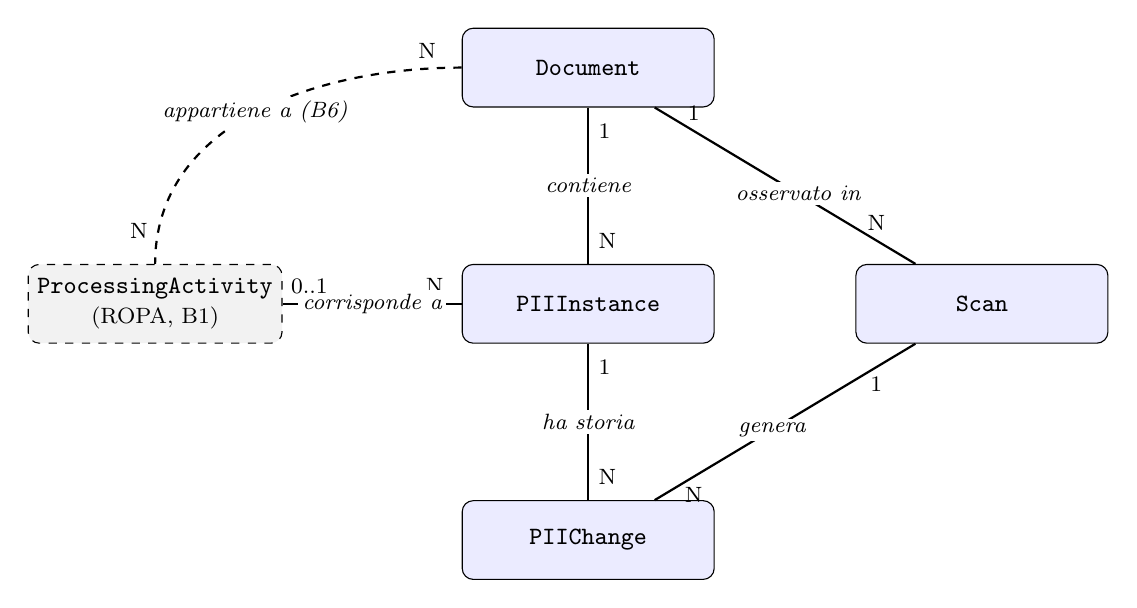
\begin{tikzpicture}[
			entity/.style={rectangle, draw, rounded corners, minimum width=3.2cm,
					minimum height=1cm, align=center, fill=blue!8, font=\small},
			ext/.style={rectangle, draw, dashed, rounded corners, minimum width=3.2cm,
					minimum height=1cm, align=center, fill=gray!10, font=\small},
			rel/.style={font=\footnotesize\itshape, fill=white, inner sep=1.5pt},
			card/.style={font=\footnotesize},
			link/.style={thick},
		]
		\node (doc)  [entity] at (0, 3)    {\texttt{Document}};
		\node (inst) [entity] at (0, 0)    {\texttt{PIIInstance}};
		\node (chg)  [entity] at (0, -3)   {\texttt{PIIChange}};
		\node (scan) [entity] at (5, 0)    {\texttt{Scan}};
		\node (act)  [ext]    at (-5.5, 0) {\texttt{ProcessingActivity}\\{\footnotesize(ROPA, B1)}};

		% Document (1)--(N) PIIInstance : contiene
		\draw [link] (doc) -- node[card, pos=0.15, right]{1}
		node[rel]{contiene} node[card, pos=0.85, right]{N} (inst);
		% PIIInstance (1)--(N) PIIChange : ha storia
		\draw [link] (inst) -- node[card, pos=0.15, right]{1}
		node[rel]{ha storia} node[card, pos=0.85, right]{N} (chg);
		% Document (1)--(N) Scan : osservato in
		\draw [link] (doc) -- node[card, pos=0.15, above]{1}
		node[rel, pos=0.55]{osservato in} node[card, pos=0.85, above]{N} (scan);
		% Scan (1)--(N) PIIChange : genera
		\draw [link] (scan) -- node[card, pos=0.15, below]{1}
		node[rel, pos=0.55]{genera} node[card, pos=0.85, below]{N} (chg);
		% PIIInstance (N)--(0..1) ProcessingActivity : corrisponde a
		\draw [link] (inst) -- node[card, pos=0.15, above]{N}
		node[rel]{corrisponde a} node[card, pos=0.85, above]{0..1} (act);
		% Document (N)--(N) ProcessingActivity : appartiene a (associazione B6, N:N)
		\draw [link, dashed] (doc) to[out=180, in=90]
		node[card, pos=0.08, above]{N}
		node[rel, pos=0.5]{appartiene a (B6)}
		node[card, pos=0.92, left]{N} (act);
	\end{tikzpicture}
	\caption[Diagramma ER del registro delle PII rilevate]{Diagramma entità--relazione del registro delle PII rilevate (blocco B5): lo stato corrente (\texttt{PIIInstance}) e la sua storia (\texttt{PIIChange}), legati alle scansioni (\texttt{Scan}) e ai documenti (\texttt{Document}). I legami con \texttt{ProcessingActivity} del registro ROPA (tratteggiati, blocco B1) sono due: l'associazione \emph{documento--trattamento} (N:N, blocco B6), registrata su \texttt{Document.activity\_ids} con la sua provenienza (\texttt{association\_source}); e il riferimento \emph{per singola PII} (0..1) a un trattamento giustificante, la cui assenza segnala una PII \emph{orfana}, popolato dalla verifica di conformità (B7) a partire dall'associazione stessa. Non mostrata la tabella delle regole cartella→trattamento (\texttt{registry\_folder\_rule}, B6), che alimenta l'associazione per prefisso.}
	\label{fig:er-registro-pii}
\end{figure}

\section{Associazione e verifica di conformità}
\label{sec:conformita}

I blocchi B6 e B7 della Figura~\ref{fig:architettura-macro-blocchi} sono il punto in cui le due metà del sistema --- il \emph{dichiarato} (il ROPA, §\ref{sec:modello-ropa}) e il \emph{rilevato} (il registro delle PII, §\ref{sec:persistenza-registro}) --- si incontrano e producono il \textbf{verdetto di conformità}. Fino a questo punto il sistema sa, separatamente, quali categorie un trattamento \emph{dichiara} e quali PII un documento \emph{contiene}; è il confronto fra i due insiemi a trasformare un rilevatore di PII in uno strumento di \emph{governance}, ed è ciò che distingue il progetto dagli strumenti di sola rilevazione (§\ref{sec:sintesi-gap}).

\subsection{Associazione documento--trattamento (B6)}
\label{sub:b6-associazione}

Il confronto ha senso solo rispetto a un termine di paragone: prima di chiedersi «questo documento è conforme?», bisogna sapere \emph{a quale trattamento} il documento appartiene. È il compito del blocco B6: associare un documento a una o più \texttt{ProcessingActivity} dichiarate.

L'associazione è \textbf{esplicita} --- la stabilisce il DPO, non un'inferenza automatica --- e la scelta è metodologica, non di comodo. Un'associazione \emph{per contenuto}, che attribuisse il documento al trattamento i cui dati dichiarati somigliano di più a quelli rilevati, sarebbe \textbf{circolare}: sceglierebbe per costruzione il trattamento che rende il documento «il più conforme possibile», svuotando di senso la verifica successiva. L'associazione esplicita mantiene invece il confronto \textbf{onesto}: il trattamento è deciso da un umano, e B7 misura poi, senza sconti, ciò che quel trattamento dichiara rispetto a ciò che il documento contiene. L'associazione resta comunque dietro un contratto (\texttt{ActivityAssigner}), così un proponente automatico o assistito dall'AI potrà in futuro \emph{proporre} l'attribuzione lasciando al DPO la conferma --- lo stesso schema \emph{human-in-the-loop} già adottato per la mappatura del ROPA (§\ref{sub:ropa-ai}).

La relazione è \textbf{molti-a-molti}: un documento può rientrare in più trattamenti (un modulo usato tanto nella selezione del personale quanto nelle paghe) e un trattamento raccoglie molti documenti. L'insieme dei trattamenti di un documento è registrato sul documento stesso (\texttt{Document.activity\_ids}); poiché ROPA e registro delle PII vivono su basi dati separate (§\ref{sec:persistenza-registro}), gli identificatori di trattamento fanno da collegamento \emph{logico} fra i due mondi, senza chiave esterna fisica.

Perché l'associazione esplicita sia \textbf{praticabile su cartelle reali} --- dove attribuire un documento alla volta è improponibile --- il DPO dispone di due modalità, entrambe \emph{decise da lui}: l'associazione \textbf{diretta} di un singolo documento e le \textbf{regole cartella→trattamento}, con cui mappa una volta un \emph{prefisso di percorso} a uno o più trattamenti; ogni documento che ricade sotto quel prefisso --- i file nuovi inclusi, alla scansione successiva --- \emph{eredita} l'associazione. Una regola non è un'inferenza per contenuto (che si è appena esclusa perché circolare): resta una scelta esplicita del DPO, solo espressa per \emph{collocazione} anziché documento per documento. La \textbf{provenienza} di ogni associazione è tracciata (\texttt{association\_source}, con valori \texttt{MANUAL} e \texttt{RULE}) e il manuale \textbf{prevale}: riapplicare le regole non sovrascrive mai un'associazione fatta a mano. Le regole si applicano come passo separato \emph{dopo} la scansione, così una scansione schedulata associa da sé i documenti nuovi --- un passo verso l'autonomia «dai una cartella e fa da solo».

\subsection{Il confronto dichiarato--rilevato e il suo vocabolario (B7)}
\label{sub:b7-vocabolario}

Fissata l'associazione, la verifica di conformità è un'operazione \textbf{insiemistica}. Da un lato l'insieme dei \texttt{pii\_type} \emph{dichiarati}: l'unione delle categorie dichiarate da \emph{tutti} i trattamenti a cui il documento è associato. Quali mappature concorrano a formare quell'insieme è un parametro esplicito del confronto: il verdetto \emph{autorevole} considera le sole mappature confermate dal DPO (§\ref{sub:ropa-ai}), mentre la consultazione interattiva conta anche quelle ancora proposte, così da restare informativa prima che la revisione del registro sia stata completata. La distinzione va tenuta presente nel leggere un verdetto, perché la stessa categoria può risultare orfana nell'una lettura e coperta nell'altra; ciò che invece non è ammissibile è che i due criteri convivano \emph{dentro} un medesimo verdetto, e la regola su quali categorie contino è perciò definita in un unico punto e usata da tutti i controlli, conservazione inclusa. Dall'altro l'insieme dei \texttt{pii\_type} \emph{rilevati}: i tipi delle PII effettivamente presenti nel documento secondo il registro. Confrontando i due insiemi, ogni tipo ricade in una voce di un \textbf{vocabolario chiuso}, che è il linguaggio con cui il sistema riporta il verdetto al DPO:

\begin{description}
	\item[Coperta] un tipo \emph{rilevato} che è anche \emph{dichiarato} da almeno uno dei trattamenti associati. È il caso conforme: il dato presente è previsto dal registro.
	\item[Orfana] un tipo \emph{rilevato} che \textbf{nessuno} dei trattamenti associati dichiara. È il segnale di conformità cardine: un dato personale presente nel documento che il ROPA non prevede --- un trattamento di fatto non dichiarato (art.~30 GDPR, art.~12 nLPD). Si dice «orfana» perché priva di un trattamento-genitore che la giustifichi.
	\item[Mancante] un tipo \emph{dichiarato} da un trattamento associato ma \textbf{non} riscontrato nel documento. Non è di per sé una violazione: può indicare una sovra-dichiarazione, oppure semplicemente che quel documento non contiene quel dato.
	\item[Non risolvibile] una categoria \emph{dichiarata} nel ROPA che non si risolve in alcun \texttt{pii\_type} (insieme vuoto, §\ref{sub:ropa-modello}): è dichiarata ma non rilevabile dal motore. Resta esplicita e va segnalata al DPO, invece di essere scambiata per conforme.
\end{description}

Sotto la cardinalità molti-a-molti la definizione di orfana è deliberatamente \textbf{permissiva}: un tipo è orfano solo se \emph{nessuno} dei trattamenti associati lo dichiara (unione, non intersezione). Un dato coperto anche da un solo trattamento pertinente è giustificato. Specularmente, a ogni singola PII rilevata la verifica assegna il primo trattamento associato che ne dichiara il tipo come «trattamento giustificante» (\texttt{processing\_activity\_id}), oppure nessuno se la PII è orfana: è il momento in cui il riferimento opzionale (0..1) lasciato vuoto dal registro (§\ref{sub:persistenza-modello-dati}) viene finalmente popolato.

Due principi ereditati dal resto del sistema governano la lettura del verdetto. Il primo è \textbf{recall-first} (§\ref{sub:b4-merge}): il sistema preferisce segnalare un'orfana di troppo che mancarne una, perché un falso positivo costa al DPO una verifica, mentre una PII non dichiarata e non vista è un rischio invisibile. Il secondo è che il verdetto è un \textbf{segnale, non una sentenza}: un'orfana afferma «non risulta dichiarata», non «è certamente una violazione». Può infatti nascere da una violazione reale oppure da un buco di mappatura a monte --- una categoria del ROPA non ancora risolta sul tipo corrispondente. È il DPO, \emph{human-in-the-loop}, a chiudere il giudizio; il sistema gli mette davanti l'evidenza strutturata.

\subsection{Verifica della conservazione}
\label{sub:b7-retention}

Alla verifica delle categorie si affianca un controllo di \textbf{conservazione} (\textit{retention}): un dato può essere legittimamente dichiarato eppure trattenuto oltre il periodo consentito. Il ROPA porta, a livello di macro-categoria, una durata massima \emph{calcolabile a macchina} (\texttt{retention\_months}, §\ref{sub:ropa-modello}); confrontandola con l'età del documento si segnala una categoria conservata oltre il limite quando un suo dato è ancora presente. La misura dell'età resta una \textbf{stima}, ma dichiarata: la data di riferimento del documento è ricavata dai metadati interni del file quando li possiede (\texttt{modDate} di un PDF, \emph{core properties} dei formati Office) e, in loro assenza, dalla sua ultima modifica sul file system (il \emph{mtime}). Poiché le due fonti non valgono lo stesso --- il \emph{mtime} è azzerato da qualunque copia massiva o ripristino da backup --- il sistema conserva accanto alla data la sua \textbf{provenienza} (§\ref{sec:sv-reference-date}) e la espone nel verdetto, così che una segnalazione fondata su un metadato interno non venga confusa con un indizio da verificare. Sono inoltre distinti due esiti che il primo prototipo confondeva: la \emph{violazione}, quando il documento eccede un termine dichiarato, e la \emph{conservazione non verificabile}, quando il registro esprime un criterio anziché una durata --- caso in cui il silenzio non deve essere scambiato per conformità. Il verdetto è infine consultabile sull'intero corpus, ordinato per mesi di sforamento, e non soltanto documento per documento.

\section{Interfaccia e restituzione al DPO}
\label{sec:report-b8}

Il blocco B8 chiude la catena: rende consultabile ciò che i blocchi precedenti hanno prodotto. La scelta architetturale che lo caratterizza è che il sistema si presenta come una \textbf{applicazione web unica}, servita su una sola porta, e non come una raccolta di comandi da terminale. La ragione è di destinatario: il DPO non è necessariamente una figura tecnica, e uno strumento di conformità utilizzabile solo da chi sa invocare un comando resta, di fatto, inutilizzato. Le interfacce a riga di comando continuano a esistere e sono pienamente funzionali, ma il loro ruolo è quello di strumenti di servizio --- automazione, esecuzioni schedulate, diagnostica --- non di via d'accesso ordinaria.

\paragraph{Una sola applicazione, due interfacce.} La revisione del registro dei trattamenti (B1) e il cruscotto di conformità nascono come applicazioni distinte, con cicli di vita e destinatari in parte diversi; sono però \emph{montate} nella stessa applicazione, che le espone sotto percorsi differenti. Il risultato è un unico servizio da avviare e configurare --- coerente con il requisito di semplicità di installazione (§\ref{sub:facilita-installazione}) --- senza che le due parti debbano fondersi in un solo componente: ciascuna conserva il proprio insieme di pagine e i propri test.

\paragraph{Consultare non deve modificare.} Il cruscotto calcola il verdetto di conformità nel momento in cui una pagina viene aperta, e questo pone un vincolo preciso: la sola consultazione non deve produrre effetti sullo stato del sistema. Il verdetto mostrato in lettura è quindi calcolato in modalità \emph{non persistente}, mentre la scrittura degli esiti per singola PII avviene soltanto in risposta a un'azione esplicita del DPO --- tipicamente l'associazione di un documento a un trattamento. È una distinzione che vale la pena rendere esplicita, perché il medesimo calcolo serve due scopi diversi: informare e registrare.

\paragraph{Riferimenti, mai valori.} La minimizzazione del dato (§\ref{sub:minimizzazione}) non è un vincolo della sola persistenza ma attraversa anche la restituzione: le PII sono presentate al DPO come \emph{riferimenti} --- categoria, posizione nel documento, provenienza del rilevamento, stato di conformità --- e in nessuna schermata compare il valore del dato personale rilevato. Un cruscotto che mostrasse i valori trasformerebbe lo strumento di verifica in una nuova copia dei dati da proteggere, vanificando la scelta compiuta a monte nel registro.

\paragraph{Due letture, per documento e per corpus.} La restituzione è organizzata su due livelli complementari. La vista \emph{per documento} risponde alla domanda «questo file è in regola?» e riunisce in un solo luogo le PII rilevate, l'associazione ai trattamenti e il verdetto. Le viste \emph{per corpus} rispondono invece alle domande che un responsabile pone su un intero archivio --- che cosa è oltre il termine di conservazione, quali documenti nessuna regola ha ancora associato --- e sono ciò che rende lo strumento praticabile su volumi reali, dove l'esame documento per documento non è una procedura eseguibile.
